\begin{frame}{Redes recurrentes. Celdas LSTM}
	\begin{columns}
		\column[]{0.45\textwidth}
		{
			\begin{itemize}
				\item Redes \textbf{recurrentes} \arrowTikz{0} Las redes neuronales recurrentes son aquellas que retienen información de sus estados anteriores y ante los mismos estímulos de entrada no siempre producen las mismas salidas, debido al estado de la celda.
			\end{itemize}
		}
		\column[]{0.45\textwidth}
		{
			\begin{figure}[ht!]
				\centering
				\resizebox{0.9\textwidth}{!}{
					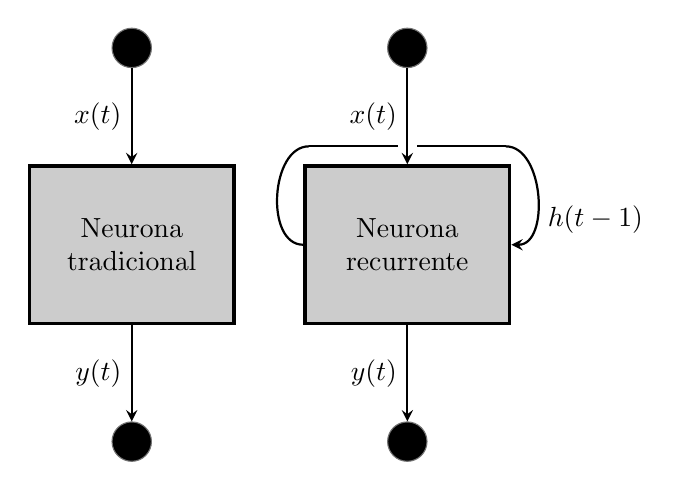
\begin{tikzpicture}
					\tikzstyle{box} = [draw,inner sep=7,minimum size=57,line 
					width=1, very thick, draw=black, fill=black!20, text width=60pt, text centered]
					\tikzstyle{stealth} = [-stealth, thick]
					\tikzstyle{invisible} = [outer sep=0,inner sep=0,minimum size=0]
					\tikzstyle{circle} = [shape=circle, minimum size=0.5cm, draw=black!55]
					\tikzstyle{line} = [draw, very thick, red]
					
					\begin{scope}
					\node [box] (v2) at (0,0) {Neurona tradicional};
					\node [circle, fill] (v1) at (0,2.5) {};
					\node [circle, fill] (v3) at (0,-2.5) {};
					\draw [stealth] (v1) edge node[anchor=east] {$x(t)$} (v2);
					\draw [stealth] (v2) edge node[anchor=east] {$y(t)$} (v3);
					\end{scope}
					\begin{scope}[shift={(3.5,0)}]
					\node [box] (v2_1) at (0,0) {Neurona recurrente};
					\node [circle, fill] (v1_1) at (0,2.5) {};
					\node [circle, fill] (v3_1) at (0,-2.5) {};
					\draw [stealth] (v1_1) edge node [anchor=east] {$x(t)$} (v2_1);
					\draw [stealth] (v2_1) edge node [anchor=east] {$y(t)$} (v3_1);
					\end{scope}
					
					\node [invisible, anchor=east] (v5) at (4.75,1.25) {};
					\draw [stealth, in =0, out=0] (v5) edge node[anchor=north west] {$h(t-1)$} (v2_1);
					\node [invisible] (v4) at (2.25,1.25) {};
					\node [] (v6) at (3.5,1.25) {};
					\draw [thick, in =180, out=180] (v2_1) edge (v4);
					\draw [thick] (v4) edge (v6);
					\draw [thick] (v6) edge (v5);
					\end{tikzpicture}
				}      
				\caption{Comparación de neuronas tradicionales con neuronas recurrentes}
				\label{fig: nn_vs_rnn}
			\end{figure}
		}
	\end{columns}
	\begin{itemize}
		\item Celdas LSTM (Long Short-Term Memory)
		\begin{itemize}
			\item \scriptsize{Propuestas por Sepp Hochreiter y Jürgen Schmidhuber en 1997.}
			\item \scriptsize{Evitan el problema de las dependencias a largo plazo.}
		\end{itemize}
	\end{itemize}
	\vspace*{-5pt}
	\begin{figure}[ht!]
		\centering
		\resizebox{0.8\textwidth}{!}{
			\begin{tikzpicture}
			\tikzstyle{box} = [draw,minimum size=15,line width=1, very thick, draw=black, fill=black!30, text centered]
			\tikzstyle{stealth} = [-stealth, thick]
			\tikzstyle{invisible} = [outer sep=0,inner sep=0,minimum size=0]
			\tikzstyle{circle} = [shape=ellipse, minimum size=15pt, draw=black!, text width=15pt, text centered]
			\tikzstyle{circle_op} = [shape=circle, minimum size=0.5cm, draw=black, very thick, fill=black!10]
			\tikzstyle{line} = [draw, very thick, red]
			\begin{scope}
			\node [circle] (v14) at (-2.25,-0.75) {$x_t$};
			\node [box] (v1) at (-1.5,0.5) {$\sigma$};
			\node [box] (v3) at (-0.5,0.5) {$\sigma$};
			\node [box] (v8) at (0.5,0.5) {$\tanh$};
			\node [box] (v6) at (1.5,0.5) {$\sigma$};
			\node [circle_op] (v2) at (-1.5,2.5) {x};
			\node [circle_op] (v4) at (0.5,1.5) {x};
			\node [circle_op] (v5) at (0.5,2.5) {\scriptsize$+$};
			\node [circle_op] (v7) at (2.5,1.25) {x};
			\node [ellipse, draw, very thick, fill=black!10] (v13) at (2.5,2) {$\tanh$};
			\draw [stealth] (v1) edge (v2);
			\draw [stealth,out=90,in=180] (v3) edge (v4);
			\draw [stealth] (v4) edge (v5);
			\draw [stealth,out=90,in=180] (v6) edge (v7);
			\node [invisible] (v11) at (-2,0) {};
			\node [invisible] (v10) at (-0.5,0) {};
			\node [invisible] (v9) at (0.5,0) {};
			\node [invisible] (v12) at (1,0) {};
			\draw [thick] (v8) edge (v4);
			\draw [thick,] (v9) edge (v8);
			\draw [thick] (v10) edge (v3);
			\draw [thick] (v11) edge (v12);
			\draw [thick,out=0,in=270] (v12) edge (v6);
			\draw [thick] (v7) edge (v13);
			\draw [thick] (v2) edge (v5);
			\draw [thick,out=90,in=180] (v14) edge (v11);
			\draw [thick,out=0,in=270] (v11) edge (v1);
			\node [invisible] (v22) at (-2.75,0) {};
			\node [invisible] (v21) at (-2.75,2.5) {};
			\node [invisible] (v17) at (4,2.5) {};
			\node [circle] (v19) at (3.5,4) {$h_t$};
			\node [invisible] (v16) at (4,0) {};
			\node [invisible] (v15) at (3,0) {};
			\draw [stealth] (v15) edge (v16);
			\draw [stealth] (v5) edge (v17);
			\node (v18) at (3.5,2.5) {};
			\draw [stealth] (v18) edge (v19);
			\node [invisible] (v20) at (3.5,0) {};
			\draw [thick] (v20) edge (v18);
			\draw [thick,out=270,in=180] (v7) edge (v15);
			\draw [thick] (v21) edge (v2);
			\draw [thick] (v22) edge (v11);
			\node [invisible] (v23) at (2.5,2.5) {};
			\draw [thick] (v13) edge (v23);
			\draw [rounded corners=2ex] (-2.75,3) rectangle (3.75,-0.25);
			\end{scope}
			\begin{scope}[shift={(6.75,0)}]
			\node [circle] (v14) at (-2.25,-0.75) {$x_{t+1}$};
			\node [box] (v1) at (-1.5,0.5) {$\sigma$};
			\node [box] (v3) at (-0.5,0.5) {$\sigma$};
			\node [box] (v8) at (0.5,0.5) {$\tanh$};
			\node [box] (v6) at (1.5,0.5) {$\sigma$};
			\node [circle_op] (v2) at (-1.5,2.5) {x};
			\node [circle_op] (v4) at (0.5,1.5) {x};
			\node [circle_op] (v5) at (0.5,2.5) {\scriptsize$+$};
			\node [circle_op] (v7) at (2.5,1.25) {x};
			\node [ellipse, draw, very thick, fill=black!10] (v13) at (2.5,2) {$\tanh$};
			\draw [stealth] (v1) edge (v2);
			\draw [stealth,out=90,in=180] (v3) edge (v4);
			\draw [stealth] (v4) edge (v5);
			\draw [stealth,out=90,in=180] (v6) edge (v7);
			\node [invisible] (v11) at (-2,0) {};
			\node [invisible] (v10) at (-0.5,0) {};
			\node [invisible] (v9) at (0.5,0) {};
			\node [invisible] (v12) at (1,0) {};
			\draw [thick] (v8) edge (v4);
			\draw [thick,] (v9) edge (v8);
			\draw [thick] (v10) edge (v3);
			\draw [thick] (v11) edge (v12);
			\draw [thick,out=0,in=270] (v12) edge (v6);
			\draw [thick] (v7) edge (v13);
			\draw [thick] (v2) edge (v5);
			\draw [thick,out=90,in=180] (v14) edge (v11);
			\draw [thick,out=0,in=270] (v11) edge (v1);
			\node [invisible] (v22) at (-2.75,0) {};
			\node [invisible] (v21) at (-2.75,2.5) {};
			\node [invisible] (v17) at (4,2.5) {};
			\node [circle] (v19) at (3.5,4) {$h_{t+1}$};
			\node [invisible] (v16) at (4,0) {};
			\node [invisible] (v15) at (3,0) {};
			\draw [stealth] (v15) edge (v16);
			\draw [stealth] (v5) edge (v17);
			\node (v18) at (3.5,2.5) {};
			\draw [stealth] (v18) edge (v19);
			\node [invisible] (v20) at (3.5,0) {};
			\draw [thick] (v20) edge (v18);
			\draw [thick,out=270,in=180] (v7) edge (v15);
			\draw [thick] (v21) edge (v2);
			\draw [thick] (v22) edge (v11);
			\node [invisible] (v23) at (2.5,2.5) {};
			\draw [thick] (v13) edge (v23);
			\draw [rounded corners=2ex,fill=black!60,opacity=0.8] (-2.75,3) rectangle (3.75,-0.25);
			\end{scope}
			\begin{scope}[shift={(-6.75,0)}]
			\node [circle] (v14) at (-2.25,-0.75) {$x_{t-1}$};
			\node [box] (v1) at (-1.5,0.5) {$\sigma$};
			\node [box] (v3) at (-0.5,0.5) {$\sigma$};
			\node [box] (v8) at (0.5,0.5) {$\tanh$};
			\node [box] (v6) at (1.5,0.5) {$\sigma$};
			\node [circle_op] (v2) at (-1.5,2.5) {x};
			\node [circle_op] (v4) at (0.5,1.5) {x};
			\node [circle_op] (v5) at (0.5,2.5) {\scriptsize$+$};
			\node [circle_op] (v7) at (2.5,1.25) {x};
			\node [ellipse, draw, very thick, fill=black!10] (v13) at (2.5,2) {$\tanh$};
			\draw [stealth] (v1) edge (v2);
			\draw [stealth,out=90,in=180] (v3) edge (v4);
			\draw [stealth] (v4) edge (v5);
			\draw [stealth,out=90,in=180] (v6) edge (v7);
			\node [invisible] (v11) at (-2,0) {};
			\node [invisible] (v10) at (-0.5,0) {};
			\node [invisible] (v9) at (0.5,0) {};
			\node [invisible] (v12) at (1,0) {};
			\draw [thick] (v8) edge (v4);
			\draw [thick,] (v9) edge (v8);
			\draw [thick] (v10) edge (v3);
			\draw [thick] (v11) edge (v12);
			\draw [thick,out=0,in=270] (v12) edge (v6);
			\draw [thick] (v7) edge (v13);
			\draw [thick] (v2) edge (v5);
			\draw [thick,out=90,in=180] (v14) edge (v11);
			\draw [thick,out=0,in=270] (v11) edge (v1);
			\node [invisible] (v22) at (-2.75,0) {};
			\node [invisible] (v21) at (-2.75,2.5) {};
			\node [invisible] (v17) at (4,2.5) {};
			\node [circle] (v19) at (3.5,4) {$h_{t-1}$};
			\node [invisible] (v16) at (4,0) {};
			\node [invisible] (v15) at (3,0) {};
			\draw [stealth] (v15) edge (v16);
			\draw [stealth] (v5) edge (v17);
			\node (v18) at (3.5,2.5) {};
			\draw [stealth] (v18) edge (v19);
			\node [invisible] (v20) at (3.5,0) {};
			\draw [thick] (v20) edge (v18);
			\draw [thick,out=270,in=180] (v7) edge (v15);
			\draw [thick] (v21) edge (v2);
			\draw [thick] (v22) edge (v11);
			\node [invisible] (v23) at (2.5,2.5) {};
			\draw [thick] (v13) edge (v23);
			\draw [rounded corners=2ex,fill=black!60,opacity=0.8] (-2.75,3) rectangle (3.75,-0.25);
			\end{scope}
			\end{tikzpicture}
		}
		\vspace*{-5pt}
		\caption{Celdas LSTM}
		\label{fig: lstm}
	\end{figure}
\end{frame}